\section{Win32 PE}
\label{win32_pe}
\myindex{Windows!Win32}

\acs{PE} это формат исполняемых файлов, принятый в Windows.

Разница между .exe, .dll, и .sys в том, что у .exe и .sys обычно нет экспортов, только импорты.

\myindex{OEP}
У \ac{DLL}, как и у всех PE-файлов, есть точка входа (\ac{OEP})
(там располагается функция DllMain()), но обычно эта функция ничего не делает.

.sys это обычно драйвера устройств.

Для драйверов, Windows требует, чтобы контрольная сумма в PE-файле была проставлена и была верной\footnote{Например, Hiew(\myref{Hiew}) умеет её подсчитывать}.

\myindex{Windows!Windows Vista}
А начиная с Windows Vista, файлы драйверов должны быть также подписаны при помощи электронной подписи, иначе они не будут загружаться.


\myindex{MS-DOS}
В начале всякого PE-файла есть крохотная DOS-программа,
выводящая на консоль сообщение вроде \q{This program cannot be run in DOS mode.} --- если запустить эту программу в DOS либо Windows 3.1 (\ac{OS} не знающие о PE-формате), 
выведется это сообщение.

\subsection{Терминология}

\begin{itemize}
\item
Модуль --- это отдельный файл, .exe или .dll.

\item Процесс --- это некая загруженная в память и работающая программа.
Как правило состоит из одного .exe-файла и массы .dll-файлов.

\item Память процесса --- память с которой работает процесс.
У каждого процесса --- своя.
Там обычно имеются загруженные модули, память стека, \glslink{heap}{кучи}, итд.

\item
\myindex{VA}
\ac{VA} --- это адрес, который будет использоваться в самой программе во время исполнения.

\item
\myindex{Базовый адрес}
Базовый адрес (модуля) --- это адрес, по которому модуль должен быть загружен в пространство процесса.

Загрузчик \ac{OS} может его изменить, если этот базовый адрес уже занят другим модулем, загруженным перед ним.

\item
\myindex{RVA}
\ac{RVA} --- это \ac{VA}-адрес минус базовый адрес. Многие адреса в таблицах PE-файла используют \ac{RVA}-адреса.

%\item
%Data directory\EMDASH{}...

\item 
\myindex{Windows!IAT}
\ac{IAT} --- массив адресов импортированных символов \footnote{\cite{Pietrek1}}. 
Иногда, директория \TT{IMAGE\_DIRECTORY\_ENTRY\_IAT} указывает на \ac{IAT}. 
\label{IDA_idata} Важно отметить, что \ac{IDA} (по крайней мере 6.1) может выделить псевдо-секцию с именем \TT{.idata} для \ac{IAT}, даже если \ac{IAT} является частью совсем другой секции!

\item 
\myindex{Windows!INT}
\ac{INT} --- массив имен символов для импортирования \footnote{\cite{Pietrek1}}.
\end{itemize}

\subsection{Базовый адрес}

Дело в том, что несколько авторов модулей могут готовить DLL-файлы для других, и нет возможности договориться о том, какие адреса и кому будут отведены.

Поэтому, если у двух необходимых для загрузки процесса DLL одинаковые базовые адреса,
одна из них будет загружена по этому базовому адресу, 
а вторая --- по другому свободному месту в памяти процесса, и все виртуальные адреса во второй DLL будут скорректированы.

\par Очень часто линкер в \ac{MSVC} генерирует .exe-файлы с базовым адресом  \TT{0x400000}\footnote{Причина выбора такого адреса описана здесь: \href{http://go.yurichev.com/17041}{MSDN}},
и с секцией кода начинающейся с \TT{0x401000}.
Это значит, что \ac{RVA} начала секции кода --- \TT{0x1000}.
А \ac{DLL} часто генерируются MSVC-линкером с базовым адресом \TT{0x10000000}\footnote{Это можно изменять опцией /BASE в линкере}.

\myindex{ASLR}
Помимо всего прочего, есть еще одна причина намеренно загружать модули по разным адресам, а точнее, по случайным.

Это \ac{ASLR}\footnote{\href{http://go.yurichev.com/17042}{wikipedia}}.

\myindex{Shellcode}
Дело в том, что некий шеллкод, пытающийся исполниться на зараженной системе, должен вызывать какие-то системные функции, а следовательно, знать их адреса.

И в старых \ac{OS} (в линейке \gls{Windows NT}: до Windows Vista),
системные DLL (такие как kernel32.dll, user32.dll) загружались все время
по одним и тем же адресам, 
а если еще и вспомнить, что версии этих DLL редко менялись, то адреса отдельных
функций, можно сказать, фиксированы и шеллкод может вызывать их напрямую.

Чтобы избежать этого, методика \ac{ASLR}
загружает и вашу программу, и все модули ей необходимые, по случайным адресам, разным при каждом запуске.

В PE-файлах, поддержка \ac{ASLR} отмечается выставлением флага \\
\TT{IMAGE\_DLL\_CHARACTERISTICS\_DYNAMIC\_BASE} (см: [\Russinovich]).

\subsection{Subsystem}

Имеется также поле \IT{subsystem}, обычно это:

\myindex{Native API}
\begin{itemize}
\item native\footnote{Что означает, что модуль использует Native API а не Win32} (.sys-драйвер), 

\item console (консольное приложение) или

\item \ac{GUI} (не консольное).
\end{itemize}

\subsection{Версия ОС}

PE-файле также задает минимальный номер версии Windows, необходимый для загрузки модуля.

Соответствие номеров версий в файле и кодовых наименований Windows, можно посмотреть
здесь\footnote{\href{http://go.yurichev.com/17044}{wikipedia}}.

\myindex{Windows!Windows NT4}
\myindex{Windows!Windows 2000}
Например, \ac{MSVC} 2005 еще компилирует .exe-файлы запускающиеся на Windows NT4 (версия 4.00), а вот \ac{MSVC} 2008 уже нет 
(генерируемые файлы имеют версию 5.00, для запуска необходима как минимум Windows 2000).

\myindex{Windows!Windows XP}
\ac{MSVC} 2012 по умолчанию генерирует .exe-файлы версии 6.00, для запуска нужна как минимум Windows Vista. 
Хотя, изменив настройки компиляции\footnote{\href{http://go.yurichev.com/17045}{MSDN}},
можно заставить генерировать и под Windows XP.

\subsection{Секции}

Разделение на секции присутствует, по-видимому, во всех форматах исполняемых файлов.

Придумано это для того, чтобы отделить код от данных, а данные --- от константных данных.


\begin{itemize}
\item На секции кода будет стоять флаг \IT{IMAGE\_SCN\_CNT\_CODE} или \IT{IMAGE\_SCN\_MEM\_EXECUTE} --- это исполняемый код.

\item На секции данных --- флаги \IT{IMAGE\_SCN\_CNT\_INITIALIZED\_DATA}, 
\IT{IMAGE\_SCN\_MEM\_READ} и \IT{IMAGE\_SCN\_MEM\_WRITE}.

\item На пустой секции с неинициализированными данными --- \IT{IMAGE\_SCN\_CNT\_UNINITIALIZED\_DATA}, \IT{IMAGE\_SCN\_MEM\_READ} и \IT{IMAGE\_SCN\_MEM\_WRITE}.

\item А на секции с константными данными, то есть, защищенными от записи, могут быть флаги \\
\IT{IMAGE\_SCN\_CNT\_INITIALIZED\_DATA} и \IT{IMAGE\_SCN\_MEM\_READ} без \IT{IMAGE\_SCN\_MEM\_WRITE}. 
Если попытаться записать что-то в эту секцию, процесс упадет.
\end{itemize}

\myindex{TLS}
\myindex{BSS}
В PE-файле можно задавать название для секции, но это не важно.
Часто (но не всегда) секция кода называется \TT{.text}, секция данных --- \TT{.data}, константных данных --- \TT{.rdata} \IT{(readable data)}.
Еще популярные имена секций: 

\myindex{MIPS}
\begin{itemize}
\item \TT{.idata} --- секция импортов. \ac{IDA} может создавать псевдо-секцию с этим же именем: \myref{IDA_idata}.
\item \TT{.edata} --- секция экспортов (редко встречается)
\item \TT{.pdata} --- секция содержащая информацию об исключениях в Windows NT для MIPS, \ac{IA64} и x64: \myref{SEH_win64}
\item \TT{.reloc} --- секция релоков
\item \TT{.bss} --- неинициализированные данные
\item \TT{.tls} --- thread local storage (\ac{TLS})
\item \TT{.rsrc} --- ресурсы
\item \TT{.CRT} --- может присутствует в бинарных файлах, скомпилированных очень старыми версиями MSVC
\end{itemize}

Запаковщики/зашифровщики PE-файлов часто затирают имена секций, или меняют на свои.

В \ac{MSVC} можно объявлять данные в произвольно названной секции\footnote{\href{http://go.yurichev.com/17047}{MSDN}}.

Некоторые компиляторы и линкеры могут добавлять также секцию с отладочными символами 
и вообще отладочной информацией (например, MinGW).

\myindex{Windows!PDB}
Хотя это не так в современных версиях \ac{MSVC} (там принято отладочную информацию сохранять в отдельных \gls{PDB}-файлах).\\
\\
Вот как PE-секция описывается в файле:

\begin{lstlisting}
typedef struct _IMAGE_SECTION_HEADER {
  BYTE  Name[IMAGE_SIZEOF_SHORT_NAME];
  union {
    DWORD PhysicalAddress;
    DWORD VirtualSize;
  } Misc;
  DWORD VirtualAddress;
  DWORD SizeOfRawData;
  DWORD PointerToRawData;
  DWORD PointerToRelocations;
  DWORD PointerToLinenumbers;
  WORD  NumberOfRelocations;
  WORD  NumberOfLinenumbers;
  DWORD Characteristics;
} IMAGE_SECTION_HEADER, *PIMAGE_SECTION_HEADER;
\end{lstlisting}
\footnote{\href{http://go.yurichev.com/17048}{MSDN}}

\myindex{Hiew}
Еще немного терминологии: \IT{PointerToRawData} называется \q{Offset} в Hiew \AndENRU \IT{VirtualAddress} называется \q{RVA} там же.

\subsection{Релоки}
\label{subsec:relocs}

Также известны как FIXUP-ы (по крайней мере в Hiew).

Это также присутствует почти во всех форматах загружаемых и исполняемых файлов
\footnote{Даже .exe-файлы в MS-DOS}.

Исключения это динамические библиотеки явно скомпилированные с \ac{PIC} или любой другой \ac{PIC}-код.

Зачем они нужны?
Как видно, модули могут загружаться по другим базовым адресам,
но как же тогда работать с глобальными переменными, например?

Ведь нужно обращаться к ним по адресу.
Одно из решений --- это \PICcode{} (\myref{sec:PIC}).  Но это далеко не всегда удобно.

Поэтому имеется таблица релоков. 
Там просто перечислены адреса мест в модуле подлежащими коррекции при загрузке по другому базовому адресу.

% TODO тут бы пример с HIEW или objdump..
Например, по \TT{0x410000} лежит некая глобальная переменная, и вот как обеспечивается её чтение:

\begin{lstlisting}
A1 00 00 41 00         mov         eax,[000410000]
\end{lstlisting}

Базовый адрес модуля \TT{0x400000}, а \ac{RVA} глобальной переменной \TT{0x10000}.

Если загружать модуль по базовому адресу \TT{0x500000}, нужно чтобы адрес этой переменной в этой инструкции стал \TT{0x510000}.

\myindex{x86!\Instructions!MOV}
Как видно, адрес переменной закодирован в самой инструкции \TT{MOV}, после байта \TT{0xA1}.

Поэтому адрес четырех байт, после \TT{0xA1}, записывается в таблицу релоков.

Если модуль загружается по другому базовому адресу,
загрузчик \ac{OS} обходит все адреса в таблице, 
находит каждое 32-битное слово по этому адресу,
отнимает от него настоящий, оригинальный базовый адрес
(в итоге получается \ac{RVA}), и прибавляет к нему новый базовый адрес.

А если модуль загружается по своему оригинальному базовому адресу, ничего не происходит.

Так можно обходиться со всеми глобальными переменными.

Релоки могут быть разных типов, однако в Windows для x86-процессоров, тип обычно \\
\IT{IMAGE\_REL\_BASED\_HIGHLOW}.

\myindex{Hiew}
Кстати, релоки маркируются темным в Hiew, например: \figref{fig:scanf_ex3_hiew_1}.

\myindex{\olly}
\olly подчеркивает места в памяти, к которым будут применены релоки, например: \figref{fig:switch_lot_olly3}.

\subsection{Экспорты и импорты}

\label{PE_exports_imports}
Как известно, любая исполняемая программа должна как-то пользоваться сервисами \ac{OS} и прочими DLL-библиотеками.

Можно сказать, что нужно связывать функции из одного модуля (обычно DLL) и места их вызовов в другом модуле (.exe-файл или другая DLL).

Для этого, у каждой DLL есть \q{экспорты}, это таблица функций плюс их адреса в модуле.

А у .exe-файла, либо DLL, есть \q{импорты}, это таблица функций требующихся для исполнения
включая список имен DLL-файлов.

Загрузчик \ac{OS}, после загрузки основного .exe-файла, проходит по таблице импортов:
загружает дополнительные DLL-файлы, 
находит имена функций среди экспортов в DLL и прописывает их адреса в \ac{IAT} в головном .exe-модуле.

\myindex{Windows!Win32!Ordinal}
Как видно, во время загрузки, загрузчику нужно много сравнивать одни имена функций с другими,
а сравнение строк\EMDASH{}это не очень быстрая процедура, так что,
имеется также поддержка \q{ординалов} или
\q{hint}-ов, это когда в таблице импортов проставлены номера функций вместо их имен.

Так их быстрее находить в загружаемой DLL.
В таблице экспортов ординалы присутствуют всегда.

\myindex{MFC}
К примеру, программы использующие библиотеки \ac{MFC}, обычно загружают mfc*.dll по ординалам, и в таких программах, в \ac{INT}, нет имен функций \ac{MFC}.

% TODO example!
При загрузке такой программы в \IDA, она спросит у вас путь к файлу mfc*.dll,
чтобы установить имена функций.
Если в \IDA не указать путь к этой DLL, то вместо имен функций будет что-то вроде \IT{mfc80\_123}.

\subsubsection{Секция импортов}

Под таблицу импортов и всё что с ней связано иногда отводится отдельная секция 
(с названием вроде \TT{.idata}),
но это не обязательно.

Импорты --- это запутанная тема еще и из-за терминологической путаницы. Попробуем собрать всё в одно место.

\begin{figure}[H]
\centering
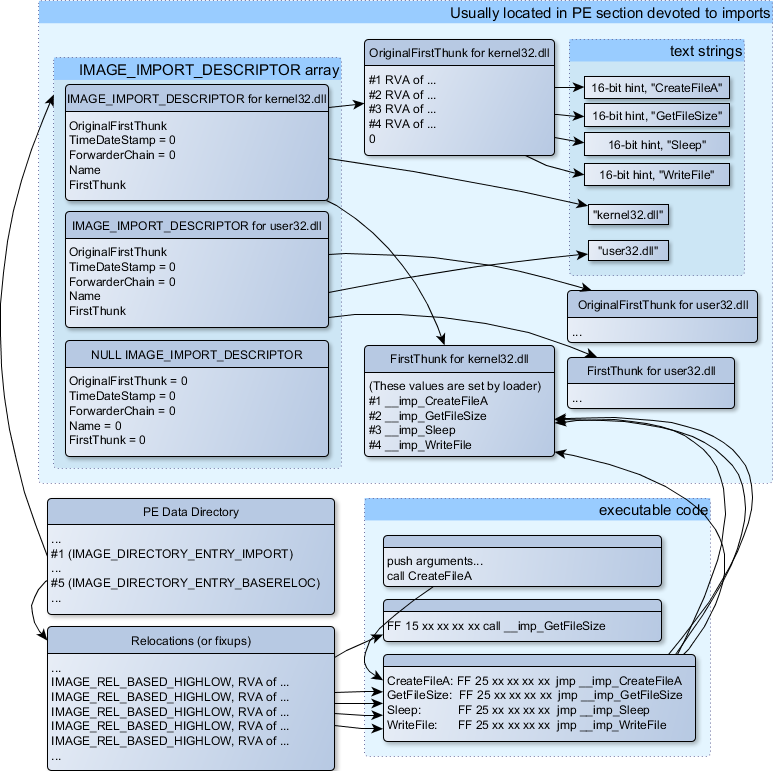
\includegraphics[scale=\FigScale]{OS/PE/unnamed0.png}
\caption{схема, объединяющая все структуры в PE-файлы, связанные с импортами}
\end{figure}

Самая главная структура --- это массив \IT{IMAGE\_IMPORT\_DESCRIPTOR}.
Каждый элемент на каждую импортируемую DLL.

У каждого элемента есть \ac{RVA}-адрес текстовой строки (имя DLL) (\IT{Name}).

\IT{OriginalFirstThink} это \ac{RVA} -адрес таблицы \ac{INT}.
Это массив \ac{RVA}-адресов, каждый из которых указывает на текстовую строку где записано имя функции. 
Каждую строку предваряет 16-битное число (\q{hint}) --- \q{ординал} функции.

Если при загрузке удается найти функцию по ординалу, тогда сравнение текстовых строк не будет происходить.
Массив оканчивается нулем.

Есть также указатель на таблицу \ac{IAT} с названием \IT{FirstThunk}, это просто \ac{RVA}-адрес места, где загрузчик будет проставлять адреса найденных функций.

Места где загрузчик проставляет адреса, \IDA именует их так: \IT{\_\_imp\_CreateFileA}, etc.

Есть по крайней мере два способа использовать адреса, проставленные загрузчиком.

\myindex{x86!\Instructions!CALL}
\begin{itemize}
\item
В коде будут просто инструкции вроде \IT{call \_\_imp\_CreateFileA}, а так как, поле с адресом импортируемой функции это как бы глобальная переменная, 
то в таблице релоков добавляется адрес (плюс 1 или 2) в инструкции \IT{call},
на случай если модуль будет загружен по другому базовому адресу.

Но как видно, это приводит к увеличению таблицы релоков.
Ведь вызовов импортируемой функции у вас в модуле может быть очень много.
К тому же, чем больше таблица релоков, тем дольше загрузка.

\myindex{x86!\Instructions!JMP}
\myindex{thunk-функции}
\item
На каждую импортируемую функцию выделяется только один переход на импортируемую функцию используя
инструкцию \JMP плюс релок на эту инструкцию.
Такие места-\q{переходники} называются также \q{thunk}-ами.
А все вызовы импортируемой функции это просто инструкция \CALL на соответствующий \q{thunk}.
В данном случае, дополнительные релоки не нужны, потому что эти CALL-ы имеют относительный адрес,
и корректировать их не надо.
\end{itemize}

Оба этих два метода могут комбинироваться.
Вероятно, линкер создает отдельный \q{thunk}, если вызовов слишком много, но по умолчанию --- не создает. \\
\\
Кстати, массив адресов функций, на который указывает FirstThunk,
не обязательно может быть в секции \ac{IAT}.
К примеру, автор сих строк написал утилиту
PE\_add\_import\footnote{\href{http://go.yurichev.com/17049}{yurichev.com}} 
для добавления импорта в уже существующий .exe-файл.
Раньше, в прошлых версиях утилиты, на месте функции, вместо которой вы хотите подставить вызов в другую DLL,
моя утилита вписывала такой код:

\begin{lstlisting}
MOV EAX, [yourdll.dll!function]
JMP EAX
\end{lstlisting}

При этом, FirstThunk указывает прямо на первую инструкцию.
Иными словами, загрузчик, загружая yourdll.dll, прописывает адрес функции \IT{function} прямо в коде.

Надо также отметить что обычно секция кода защищена от записи, так что, моя утилита добавляет флаг \\
\IT{IMAGE\_SCN\_MEM\_WRITE} 
для секции кода. Иначе при загрузке такой программы, она упадет с ошибкой 5 (access denied). \\
\\
Может возникнуть вопрос: а что если я поставляю программу с набором DLL,
которые никогда не будут меняться (в т.ч., адреса всех функций в этих DLL), может как-то можно ускорить процесс загрузки?

Да, можно прописать адреса импортируемых функций в массивы FirstThunk заранее.
Для этого в структуре \\
\IT{IMAGE\_IMPORT\_DESCRIPTOR} имеется поле \IT{Timestamp}.
И если там присутствует какое-то значение, то загрузчик сверяет это значение с датой-временем DLL-файла.
И если они равны, то загрузчик больше ничего не делает, и загрузка может происходить быстрее.

Это называется \q{old-style binding}
\footnote{\href{http://go.yurichev.com/17050}{MSDN}.
Существует также \q{new-style binding}.}.
\myindex{BIND.EXE}
В Windows SDK для этого имеется утилита BIND.EXE.
Для ускорения загрузки вашей программы, 
Matt Pietrek в \cite{Pietrek1}, предлагает делать binding сразу после инсталляции
вашей программы на компьютере конечного пользователя. \\
\\
Запаковщики/зашифровщики PE-файлов могут также сжимать/шифровать таблицу импортов.
В этом случае, загрузчик Windows, конечно же, не загрузит все нужные DLL.
\myindex{Windows!Win32!LoadLibrary}
\myindex{Windows!Win32!GetProcAddress}
Поэтому распаковщик/расшифровщик делает это сам, при помощи вызовов \IT{LoadLibrary()} и \IT{GetProcAddress()}.
Вот почему в запакованных файлах эти две функции часто присутствуют в \ac{IAT}. \\
\\
В стандартных DLL входящих в состав Windows, часто, \ac{IAT} находится в самом начале PE-файла.

Возможно это для оптимизации.
Ведь .exe-файл при загрузке не загружается в память весь 
(вспомните что инсталляторы огромного размера подозрительно быстро запускаются), он \q{мапится} (map), 
и подгружается в память частями по мере обращения к этой памяти.

И возможно в Microsoft решили что так будет быстрее.

\subsection{Ресурсы}

\label{PEresources}
Ресурсы в PE-файле\EMDASH{}это набор иконок, картинок, текстовых строк, описаний диалогов.
Возможно, их в свое время решили отделить от основного кода, чтобы все эти вещи были многоязычными,
и было проще выбирать текст или картинку того языка, который установлен в \ac{OS}. \\
\\
В качестве побочного эффекта, их легко редактировать и сохранять обратно в исполняемый файл,
даже не обладая специальными знаниями, например, редактором ResHack (\myref{ResHack}).

\subsection{.NET}

\myindex{.NET}
Программы на .NET компилируются не в машинный код, а в свой собственный байткод.
\myindex{OEP}
Собственно, в .exe-файлы байткод вместо обычного кода, однако, точка входа (\ac{OEP}) 
указывает на крохотный фрагмент x86-кода:

\begin{lstlisting}
jmp         mscoree.dll!_CorExeMain
\end{lstlisting}

А в mscoree.dll и находится .NET-загрузчик, который уже сам будет работать с PE-файлом.

\myindex{Windows!Windows XP}
Так было в \ac{OS} до Windows XP. Начиная с XP, загрузчик \ac{OS} уже сам определяет, что это
.NET-файл и запускает его не исполняя этой инструкции \JMP

\footnote{\href{http://go.yurichev.com/17051}{MSDN}}.

\myindex{TLS}
\subsection{TLS}

Эта секция содержит в себе инициализированные данные для \ac{TLS}(\myref{TLS}) (если нужно).
При старте нового треда, его \ac{TLS}-данные инициализируются данными из этой секции. \\
\\
\myindex{TLS!Callbacks}
Помимо всего прочего, спецификация PE-файла предусматривает инициализацию \ac{TLS}-секции, т.н., TLS callbacks.
Если они присутствуют, то они будут вызваны перед тем как передать управление на главную точку входа (\ac{OEP}).
Это широко используется запаковщиками/защифровщиками PE-файлов.

\subsection{Инструменты}

\begin{itemize}
\item
\myindex{objdump}
\myindex{Cygwin}
objdump (имеется в cygwin) для вывода всех структур PE-файла.

\item
\myindex{Hiew}
Hiew(\myref{Hiew}) как редактор.

\item pefile --- Python-библиотека для работы с PE-файлами
\footnote{\url{http://go.yurichev.com/17052}}.

\item
\label{ResHack}
ResHack \acs{AKA} Resource Hacker --- редактор ресурсов
\footnote{\url{http://go.yurichev.com/17052}}.

\item PE\_add\_import\footnote{\url{http://go.yurichev.com/17049}} --- простая утилита для добавления символа/-ов в таблицу импортов PE-файла.

\item PE\_patcher\footnote{\href{http://go.yurichev.com/17054}{yurichev.com}} --- простая утилита для модификации PE-файлов.

\item PE\_search\_str\_refs\footnote{\href{http://go.yurichev.com/17055}{yurichev.com}} --- простая утилита для поиска функции в PE-файле, где используется некая текстовая строка.
\end{itemize}

\subsection{Further reading}

% FIXME: bibliography per chapter or section
\begin{itemize}
\item Daniel Pistelli --- The .NET File Format \footnote{\url{http://go.yurichev.com/17056}}
\end{itemize}

